\section{Notions pr\'eliminaires}

\subsection{Automates temporis\'es}
\label{fr:sec:formal_methods}
Les automates temporisés seront utilisés dans la suite pour réaliser un modèle formel de
des architectures.
Un automate temporisé est un automate étendu permettant en outre de modéliser le temps, et ce
en ajoutant un nouveau type de variable appelé horloge. On rappelle qu'un automate étendu est un automate
pouvant manipuler des variables entières.


\begin{definition}[Horloges]
  Une \textit{horloge} est une variable modélisant le passage du temps.
  La valeur d'une horloge ne croit que dans les états car les transitions sont instantanées.
  La valeur d'une horloge peut être testée sur une garde d'une transition et remise à zéro après franchissement d'une transition.
\end{definition}


\begin{definition}[Syntaxe des contraintes et des actions]
\label{fr:def:formal_methods:transition_grammar2}
Étant donné un ensemble de variables \automatavariables{}, et un ensemble
d'horloges \automataclocks{}, la grammaire utilisée pour l'écriture des
contraintes et des actions de transitions est la suivante, avec \textbf{ident}
indiquant une variable dans \automatavariables{} et \textbf{clk} une horloge
dans \automataclocks{}:\\
$\textbf{lop} ::= \land~|~\lor $\\
$\textbf{cop} ::=\!\!\! ~< | \le | = | \ge | > $\\
$\textbf{mop} ::= +~| - | * |~/$\\
$
\textbf{val} ::=
   \textbf{ident}
   ~|~ \mathbb{Z}
$\\
$\textbf{mexpr} ::=
   \textbf{mexpr}~\textbf{mop}~\textbf{mexpr}
   ~|~ \textbf{val}
$\\
$
\textbf{abexpr} ::=
   \textbf{mexpr}~\textbf{cop}~\textbf{mexpr}
   ~|~ \textbf{clk}~\textbf{cop}~\textbf{val}
   ~|~ \textbf{clk} - \textbf{clk}~\textbf{cop}~\textbf{val}
   ~|~ \texttt{true}
   ~|~ \texttt{false}
$\\
$
\textbf{bexpr} ::=
   \neg \textbf{bexpr}
   ~|~ \textbf{bexpr}~\textbf{lop}~\textbf{bexpr}
   ~|~ \textbf{abexpr}
$\\
$\textbf{iexpr} ::=
   \textbf{iexpr} \land \textbf{iexpr}
   ~|~ \textbf{clk}~\textbf{cop}~\textbf{val}
   ~|~ \textbf{clk} - \textbf{clk}~\textbf{cop}~\textbf{val}
   ~|~ \texttt{true}
$\\
$
\textbf{assign} ::=
   \textbf{assign};~\textbf{assign}
   ~|~ \textbf{ident}~:=~\textbf{mexpr}
   ~|~ if~(\textbf{bexpr})~\{\textbf{assign}\}
   ~|~ \textbf{clk} := 0
   ~|~ \texttt{nop}
$
\end{definition}



\begin{definition}[Automates temporisés]
Un automate temporisé \automatasystem{} est un tuple
$\langle \automatastates{}, \allowbreak{}
\automatainvariants{}, \allowbreak{}
\automatainit{}, \allowbreak{}
\automatacondlabels{}, \allowbreak{}
\automatachanlabels{}, \allowbreak{}
\automatachanpriorities{}, \allowbreak{}
\automatavariables{}, \allowbreak{}
\automataclocks{}, \allowbreak{}
\automataactionlabels{}, \allowbreak{}
\automatarelations{}\rangle$ tel que:
\begin{itemize}
  \setlength{\itemsep}{0pt}%
   \setlength{\parskip}{0pt}%
\item \automatastates{} est un ensemble fini de localités.
\item
   $\automatainvariants{} : \automatastates{} \to \textbf{iexpr}$ indique
   l'invariant associé à chaque localité.
\item \automatainit{} est la localité initiale ($\automatainit{} \in
\automatastates{}$).
\item \automatavariables{} est un ensemble fini de variables.
\item \automataclocks{} est un ensemble fini d'horloges.
\item
   $\automatachanlabels{} = \automatachanlabels{}^{\alpha} \cup
   \automatachanlabels{}^{\texttt{sync}}$ est un ensemble fini d'étiquettes, avec
   $\automatachanlabels{}^{\texttt{sync}}$ correspondant aux étiquettes de
   synchronisation et $\automatachanlabels{}^{\alpha}$ aux autres.
   $\automatachanlabels{}^{\texttt{sync}} \cap \automatachanlabels{}^{\alpha}
   = \emptyset$.
   Les étiquettes dans $\automatachanlabels{}^{\texttt{sync}}$ terminent soit par
   par `?' qui indique la réception sur un ``canal'',
   ou par `!' qui indique l'émission.
\item
   \automatacondlabels{} = \textbf{bexpr}(\automatavariables{},
   \automataclocks{}) est l'ensemble des gardes, utilisant la grammaire de
   Définition~\ref{fr:def:formal_methods:transition_grammar2}.
\item
   \automataactionlabels{} = \textbf{assign}(\automatavariables{},
   \automataclocks{}), est l'ensemble des actions, utilisant la grammaire de
   Définition~\ref{fr:def:formal_methods:transition_grammar2}.
\item
   $\automatarelations{} \subseteq
      \automatastates{}
      \times \automatacondlabels{}
      \times \automatachanlabels{}
      \times \automataactionlabels{}
      \times \automatastates{}
   $ est la relation de transition.
\end{itemize}
La sémantique de \automatasystem{} est donnée à travers ses traces d'exécution
(voir Définition~\ref{fr:def:formal_methods:trace2}).
\end{definition}

\begin{definition}[Valuation d'horloge]
La fonction
$\automataclockvals{}: \automataclocks \to \mathbb{R}^+$ assigne une valuation
à chaque horloge. On note $(\automataclockvals{} + t)$ comme abréviation pour
indiquer l'incrément de la valeur de toutes les horloges dans \automataclockvals{}
de $t$ unités de temps.
\end{definition}

\begin{definition}[Valuation des variables]
  Les valuations
$\automataenvironment{}:\automatavariables{} \to \mathbb{N}$
  associent aux variables leur valeur.
Étant donné une valuation $\automataenvironment{}$ et une garde
$c \in \automatacondlabels{}$, on note $\automataenvironment{} \models_{PL} c$
pour indiquer que $c$ est vraie selon la valuation $v$.
De même, étant donné $a \in \automataactionlabels{}$, $v[a]$ correspond à la
valuation obtenue depuis $v$ par l'application de l'action $a$: toutes les
variables changées par $a$ ont leur nouvelle valeur et toutes les autres gardent
leur valeur précédente.
\end{definition}


\begin{definition}[Transition]
Étant donné un automate
$\automatasystem{} = \allowbreak{}
\langle \automatastates{}, \allowbreak{}
\automatainvariants{}, \allowbreak{}
\automatainit{}, \allowbreak{}
\automatacondlabels{}, \allowbreak{}
\automatachanlabels{}, \allowbreak{}
\automatachanpriorities{}, \allowbreak{}
\automatavariables{}, \allowbreak{}
\automataclocks{}, \allowbreak{}
\automataactionlabels{}, \allowbreak{}
\automatarelations{}\rangle$,
on définit \automatanext{} permettant de calculer l'ensemble des transitions valides depuis
$\langle \automatastate{}, \automataenvironment{}, \automataclockvals{}\rangle$,
avec
$s \in \automatastates{}$, $\automataenvironment{}$ une valuation des variables,
$\automataclockvals{}$ une valuation des horloges et $t$ le temps passé
dans la localité courante:
$\automatanext{}(\langle \automatastate{}, \automataenvironment{}, \automataclockvals{}\rangle, t)
\triangleq \{\langle \automatastate{}', \automataenvironment{}', \automataclockvals{}' \rangle
|
   \existsin{\langle \automatastate{}, c, l, a, \automatastate{}' \rangle}{\automatarelations{}}{%
%      (o = \automatastate{})
%      \land (d = \automatastate{}')
      (\langle \automataenvironment{}, (\automataclockvals{} + t) \rangle \models_{PL} c)
      \land
      \automataenvironment{}' = \automataenvironment{}[a]
      \land
      \automataclockvals{}' = (\automataclockvals{} + t)[a]
      \land
      (\langle \automataenvironment{}', \automataclockvals{}' \rangle \models_{PL} \automatainvariants{}(\automatastate{}'))
      \land
      \neg
      \existsin{\langle \automatastate{b}, c_b, l_b, a_b, \automatastate{b}' \rangle}{\automatarelations{}}{%
   %      (o = \automatastate{})
   %      \land (d = \automatastate{}')
         (\langle \automataenvironment{}, (\automataclockvals{} + t) \rangle \models_{PL} c_b)
         \land
         \automataenvironment{}'' = \automataenvironment{}[a_b]
         \land
         \automataclockvals{}'' = (\automataclockvals{} + t)[a_b]
         \land
         (\langle \automataenvironment{b}'', \automataclockvals{b}'' \rangle \models_{PL} \automatainvariants{}(\automatastate{b}'))
         \land
         (l \in \automatachanpriorities{}(l_b)) \allowbreak{}
      }
   }\}
$
\end{definition}

\begin{definition}[Chemin et trace]
\label{fr:def:formal_methods:trace2}
Un chemin est une séquence maximale de transitions\linebreak
$\langle \automatastate{0}, \automataenvironment{0}, \automataclockvals{0}\rangle
\automatatransition{}^{\!\!\!t_0} \langle \automatastate{1},
\automataenvironment{1}, \automataclockvals{1}\rangle \automatatransition{}^{\!\!\!t_{1}} \cdots$ telle que pour chaque $k$,
$\langle \automatastate{k+1}, \automataenvironment{k+1}, \automataclockvals{k+1}\rangle \in \automatanext{}(\langle \automatastate{k}, \automataenvironment{k}, \automataclockvals{k}\rangle, t_k)
$.
La séquence est maximale dans le sens où elle est soit infinie soit de longueur $N$ et telle que $\automatanext{}(\langle \automatastate{N}, \automataenvironment{N}, \automataclockvals{N}\rangle, t)$ est vide pour tout $t\in \mathbb{R}^+$. On appelle trace un chemin partant de l'état initial
$\langle
\automatainit{}, \automataenvironment{0},  \automataclockvals{0}\rangle$, avec
\automataenvironment{0} la valuation initiale et \automataclockvals{0} la valuation
telle que toutes les horloges sont à zéro.
\end{definition}


\begin{definition}[Produit synchronisé d'automates temporisés]
Étant donné \emph{n} automates temporisés
$\automatasystem{}_i = \allowbreak{}
\langle \automatastates{}_i, \allowbreak{}
\automatainvariants{}_i, \allowbreak{}
\automatainit{}_i, \allowbreak{}
\automatacondlabels{}_i, \allowbreak{}
\automatachanlabels{}_i, \allowbreak{}
\automatavariables{}_i, \allowbreak{}
\automataclocks{}, \allowbreak{}
\automataactionlabels{}_i, \allowbreak{}
\automatarelations{}_i\rangle$ et une contrainte de synchronisation
$\automatasyncconstraint{} \subseteq (\automatachanlabels{}_1 \cup \{-\})
\times \cdots \times (\automatachanlabels{}_n \cup \{-\})$,
le produit synchronisé des automates est l'automate
$\automatasystem{}_s = \allowbreak{}
\langle \automatastates{}_s, \allowbreak{}
\automatainvariants{}_s, \allowbreak{}
\automatainit{}_s, \allowbreak{}
\automatacondlabels{}_s, \allowbreak{}
\automatachanlabels{}_s, \allowbreak{}
\automatavariables{}_s, \allowbreak{}
\automataclocks{}_s, \allowbreak{}
\automataactionlabels{}_s, \allowbreak{}
\automatarelations{}\rangle$ avec:
\begin{itemize}
  \setlength{\itemsep}{0pt}%
   \setlength{\parskip}{0pt}%
\item $\automatastates{}_s =
   \automatastates{}_1 \times \cdots \times \automatastates{}_n$
\item $\automatainvariants{}_s(\automatastates{}_1 \times \cdots \times \automatastates{}_n)
   = \automatainvariants{}_1(\automatastates{}_1) \land \cdots \land \automatainvariants{}_n(\automatastates{}_n)
   $
\item $\automatainit{}_s =
   \langle{} \automatainit{}_1, \cdots, \automatainit{}_n\rangle{}$
\item $\automatacondlabels{}_s =
   \automatacondlabels{}_1 \times \cdots \times \automatacondlabels{}_n$
\item $\automatachanlabels{}_s =
(\automatachanlabels{}_1 \cup \{-\})
\times \cdots \times (\automatachanlabels{}_n \cup \{-\})$. On ajoute aux étiquettes
la notation $-$ pour indiquer qu'un sous-automate ne fait pas de transition,
\item $\automatavariables{}_s =
   \automatavariables{}_1 \cup \cdots \cup \automatavariables{}_n$,
   avec $\forallin{i,j}{1\ldots n}{(i \neq j) \implies (\automatavariables{}_i \cap \automatavariables{}_j = \emptyset)}$
\item $\automataclocks{}_s =
   \automataclocks{}_1 \cup \cdots \cup \automataclocks{}_n$
%   avec $\forallin{i,j}{1..n}{(i \neq j) \implies (\automataclocks{}_i \cap \automataclocks{}_j = \emptyset)}$.
\item $\automataactionlabels{}_s =
   \automataactionlabels{}_1 \times \cdots \times \automataactionlabels{}_n$
\item
   $\automatarelations{}_s \subseteq
      \automatastates{}_s
      \times \automatacondlabels{}_s
      \times \automatachanlabels{}_s
      \times \automataactionlabels{}_s
      \times \automatastates{}_s
   $, avec
   $$
   \langle
      \langle o_1, \cdots, o_n \rangle,
      \langle c_1, \cdots, c_n \rangle,
      \langle l_1, \cdots, l_n \rangle,
      \langle a_1, \cdots, a_n \rangle,
      \langle d_1, \cdots, d_n \rangle
   \rangle \in \automatarelations{}_s
   $$
   $$
   \iff
   \begin{cases}
      \langle l_1, \cdots, l_n \rangle \in \automatasyncconstraint{}\\
      \langle
         \forall i \in 1\ldots n :
         o_i, c_i, l_i, a_i, d_i \rangle \in \automatarelations{}_i
         \lor (o_i = d_i \land l_i = - \land c_i = \texttt{true} \land a_i =
         \textit{nop})
   \end{cases}
   $$
\end{itemize}
%% \automatasyncconstraint{} est défini de manière implicite par les étiquettes de
%% $\automatachanlabels_{1..n}$: pour toute transition avec une étiquette appartenant
%% à $\automatachanlabels^{\alpha}$, il y a une entrée dans
%% \automatasyncconstraint{} avec aucune autre transition simultanée autorisée
%% (indiqué par $-$ pour dire que le sous-automate en question ne fait pas de
%% transition). Pour toute transition $chan$ dans
%% $\automatachanlabels^{\texttt{sync}}$, \automatasyncconstraint{} a une entrée
%% pour chaque combinaison possible d'étiquette $chan!$, $chan?$ ou $-$ telle qu'il
%% n'y a qu'un seule étiquette $chan!$ et une seule étiquette  $chan?$. Cette convention
%% a été introduite dans CCS (\cite{10.5555/539036}).
La sémantique d'un produit synchronisé est exprimée comme la sémantique d'un automate.
\end{definition}

\begin{figure}[hbt]
   \centering
   \begin{tabular}{cc}
   \begin{tikzpicture}[->,>=stealth',shorten >=1pt,auto,node distance=3cm,
                    semithick]
   \node[initial,state] (S0)              {$S_0$};
   \node[state] (S1) [right of=S0] {$S_1$};

   \path[every node/.style={sloped, anchor=center, yshift=1em}]
      (S0) edge [bend left] node [above=-1em]{
      \begin{tabular}{l}
         $\textbf{request\_files}!$\\
         $\textit{first}$
         $\textit{fetched} := 0; C_0 := 0$
      \end{tabular}
      } (S1)

      (S1) edge [bend left] node [below=1em] {
      \begin{tabular}{l}
         $\textbf{done}?$\\
         $\textit{first} := \bot$
      \end{tabular}
      } (S0)

      (S1) edge [loop right] node [below=1em] {
      \begin{tabular}{l}
         $\textbf{new\_file}?$\\
         $\textit{fetched} := \textit{fetched} + 1$\\
      \end{tabular}
      } (S1)
   ;
\end{tikzpicture}
 &
   \begin{tikzpicture}[->,>=stealth',shorten >=1pt,auto,node distance=3cm,
                    semithick]
   \node[initial,state] (S0)              {$S_0$};
   \node[state,label=below:{$C_1 \le 64$}] (S1) [right of=S0] {$S_1$};

   \path[every node/.style={sloped, anchor=center, yshift=1em}]
      (S0) edge [bend left] node [above=-1em]{
      \begin{tabular}{l}
         $\textbf{request\_files}?$\\
         $\textit{sent} := 0; C_1 := 0$\\
      \end{tabular}
      } (S1)

      (S1) edge [bend left] node [below=1em] {
      \begin{tabular}{l}
         $\textbf{done}!$\\
         $\textit{sent} = 386$
      \end{tabular}
      } (S0)

      (S1) edge [loop right] node [below=1em] {
      \begin{tabular}{l}
         $\textbf{new\_file}!$\\
         $\textit{sent} < 386 \land C_1 \ge 32$\\
         $\textit{sent} := \textit{sent} + 1; C_1 := 0$
      \end{tabular}
      } (S1)
   ;
\end{tikzpicture}

   \end{tabular}
   \caption{Exemple de réseau d'automates temporisés}
   \label{fr:fig:timed_automata_urgent_comitted}
\end{figure}

\begin{example}[Automates temporisés] La
Figure~\ref{fr:fig:timed_automata_urgent_comitted} montre deux automates
modélisant un client (sur la gauche) qui récupère des fichiers depuis un
serveur (sur la droite). Dans ce scénario, le système boucle infiniment:
le client initialise une demande de fichiers (\textbf{request\_files}) et
compte (\textit{fetched}) leurs arrivées (\textbf{new\_file}) jusqu'à ce que le
serveur indique que tout a été transféré (\textbf{done}). A chaque requête, le
serveur envoie exactement 386 fichiers (comptés par \textit{sent}).  Le serveur
prend entre 32 et 64 unités de temps pour fournir chaque fichier, ce qui permet
de modéliser les temps de transfert.

Voici un extrait de trace valide pour ce réseau d'automates:\\
$
   \langle \langle S_0, S_0 \rangle,
   \{
      \langle \textit{first}, \top \rangle,
      \langle \textit{fetched}, 0 \rangle,
      \langle \textit{sent}, 0 \rangle
   \},
   \{
      \langle C_0, 0\rangle,
      \langle C_1, 0\rangle
   \}\rangle
   \automatatransitiontrace{\langle \textbf{request\_file!}, \textbf{request\_file?}\rangle}{}^{23}
   \\
   \langle \langle S_1, S_1 \rangle,
   \{
      \langle \textit{first}, \top \rangle,
      \langle \textit{fetched}, 0 \rangle,
      \langle \textit{sent}, 0 \rangle
   \},
   \{
      \langle C_0, 0\rangle,
      \langle C_1, 0\rangle
   \}\rangle
   \automatatransitiontrace{\langle \textbf{new\_file!}, \textbf{new\_file?}\rangle}{}^{12}
   \\
   \langle \langle S_1, S_1 \rangle,
   \{
      \langle \textit{first}, \top \rangle,
      \langle \textit{fetched}, 1 \rangle,
      \langle \textit{sent}, 1 \rangle
   \},
   \{
      \langle C_0, 12\rangle,
      \langle C_1, 0\rangle
   \}\rangle \allowbreak
   \automatatransitiontrace{\langle \textbf{new\_file!}, \textbf{new\_file?}\rangle}{}^{42}
   \\
   \langle \langle S_1, S_1 \rangle,
   \{
      \langle \textit{first}, \top \rangle,
      \langle \textit{fetched}, 2 \rangle,
      \langle \textit{sent}, 2 \rangle
   \},
   \{
      \langle C_0, 56\rangle,
      \langle C_1, 0\rangle
   \}\rangle \allowbreak
   \automatatransitiontrace{\langle \textbf{new\_file!}, \textbf{new\_file?}\rangle}{}^{32}\\
   \cdots\\
   \langle \langle S_1, S_1 \rangle,
   \{
      \langle \textit{first}, \top \rangle,
      \langle \textit{fetched}, 386 \rangle,
      \langle \textit{sent}, 386 \rangle
   \},
   \{
      \langle C_0, 16086\rangle,
      \langle C_1, 0\rangle
   \}\rangle \allowbreak
   \automatatransitiontrace{\langle \textbf{done?}, \textbf{done!}\rangle}{}^{46}\\
   \langle \langle S_0, S_0 \rangle,
   \{
      \langle \textit{first}, \bot \rangle,
      \langle \textit{fetched}, 386 \rangle,
      \langle \textit{sent}, 386 \rangle
   \},
   \{
      \langle C_0, 16132\rangle,
      \langle C_1, 46\rangle
   \}\rangle \allowbreak
$\\
À la fin de la trace, $C_0 - C_1$ correspond au temps de transfert total
des fichiers.
\end{example}

Un des intérêts d'une modélisation sous forme d'automates (temporisés ou non) est de donner à accès
à des outils de vérification formelle.
Ainsi, on peut définir la relation de satisfiabilité pour une
propriété $\phi$. On suppose que $\phi$ est une formule
d'un sous ensemble de CTL
(\cite{10.1145/567067.567080}).
La satisfiabilité de
$\langle \automatastate{}, \automataenvironment{} \rangle \models \phi$ est
définie en utilisant la décomposition suivante:

\begin{description}
   \setlength{\itemsep}{0pt}%
   \setlength{\parskip}{0pt}%
\item[%
   $
      \langle
         \automatastate{},
         \automataenvironment{}
      \rangle{}
      \models
      \psi
      \triangleq
   $]
   $\automataenvironment{} \models_{PL} \psi$, où $\psi$ est une
   expression dans $\textbf{abexpr}(\automatavariables{})$.
\item[%
   $
      \langle
         \automatastate{},
         \automataenvironment{}
      \rangle{}
      \models
      \neg \phi
      \triangleq
   $]
   $
      \langle
         \automatastate{},
         \automataenvironment{}
      \rangle{}
      \not\models
      \phi
   $
\item[%
   $
      \langle
         \automatastate{},
         \automataenvironment{}
      \rangle{}
      \models
      \phi \land \psi
      \triangleq
   $]
   $
      (\langle
         \automatastate{},
         \automataenvironment{}
      \rangle{}
      \models
      \phi)
   $
   et
   $(\langle
         \automatastate{},
         \automataenvironment{}
      \rangle{}
      \models
      \psi)
   $
\item[%
   $
      \langle
         \automatastate{},
         \automataenvironment{}
      \rangle{}
      \models
      \afop{}~\phi \triangleq
   $]~~\\
      Pour tous les chemins partant de
         $\langle
            \automatastate{},
            \automataenvironment{}
         \rangle$,
         il y a, dans le chemin, un
         $\langle
            \automatastate{}',
            \automataenvironment{}'
         \rangle$,
         tel que
         $\langle
            \automatastate{}',
            \automataenvironment{}'
         \rangle{}
         \models~\phi
         $
\item[%
   $
      \langle
         \automatastate{},
         \automataenvironment{}
      \rangle{}
      \models
      \efop{}~\phi \triangleq
   $]~~\\
      Il y a un chemin partant de
         $\langle
            \automatastate{},
            \automataenvironment{}
         \rangle$ dans lequel il y a un
         $\langle
            \automatastate{}',
            \automataenvironment{}'
         \rangle$,
         tel que
         $\langle
            \automatastate{}',
            \automataenvironment{}'
         \rangle{}
         \models~\phi
         $
\item[%
   $
      \langle
         \automatastate{},
         \automataenvironment{}
      \rangle{}
      \models
      \agop{}~\phi \triangleq
   $]~~\\
      Pour tous les chemins partant de
         $\langle
            \automatastate{},
            \automataenvironment{}
         \rangle$,
         tous les
         $\langle
            \automatastate{}',
            \automataenvironment{}'
         \rangle$
         du chemin vérifient
         $\langle
            \automatastate{}',
            \automataenvironment{}'
         \rangle{}
         \models~\phi
         $
\item[%
   $
      \langle
         \automatastate{},
         \automataenvironment{}
      \rangle{}
      \models
      \egop{}~\phi \triangleq
   $]~~\\
      Il y a un chemin partant de
         $\langle
            \automatastate{},
            \automataenvironment{}
         \rangle$ tel que tous les
         $\langle
            \automatastate{}',
            \automataenvironment{}'
         \rangle$
         du chemin vérifient
         $\langle
            \automatastate{}',
            \automataenvironment{}'
         \rangle{}
         \models~\phi
         $
\item[%
   $
      \langle
         \automatastate{},
         \automataenvironment{}
      \rangle{}
      \models
      \leadstoop{\phi}{\psi} \triangleq
   $]~~\\
      Pour tous les chemins partant de
         $\langle
            \automatastate{},
            \automataenvironment{}
         \rangle$,
         tout sous-chemin partant d'un
         $\langle
            \automatastate{}',
            \automataenvironment{}'
         \rangle$
         tel que
         $
         \automataenvironment{}'
         \models_{PL} \phi
         $
         contient aussi au moins un
         $\langle
            \automatastate{}'',
            \automataenvironment{}''
         \rangle$
         tel que
         $
         \automataenvironment{}''
         \models_{PL} \psi
         $.
\end{description}


\subsection{Fonctionnement des caches}
\label{fr:sec:cache_coherence}
Parmi les mécanismes complexes d'un processeur multi-coeur se trouve la cohérence de caches. Celle-ci assure que tous les
c\oe urs lisant ou écrivant dans un même bloc mémoire ne peuvent pas
aveuglement ignorer les modifications appliquées par les autres.
Afin de maintenir la cohérence de caches, le processeur suit un protocole pré-déterminé qui définit
les messages à envoyer en fonction des actions d'un c\oe ur ainsi que les actions
à effectuer lors de la réception du message d'un autre c\oe ur.
Pour comprendre ce mécanisme, commençons par présenter l'architecture générale et les composants participant à la cohérence
(présentés dans la figure \ref{fr:fig:cache-coherence-cmps}).


\begin{figure}[hbt]
\begin{center}
\begin{tabular}{cc}
\begin{subfigure}[t]{0.47\textwidth}
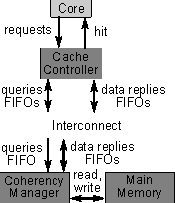
\includegraphics[width=14em]{\chapterdirectory/../cache_coherence/figure/cmp_overview.pdf}
\caption{Vue d'ensemble}%
\label{fr:fig:cache-coherence-cmps-overview}
\end{subfigure} &
\begin{subfigure}[t]{0.47\textwidth}
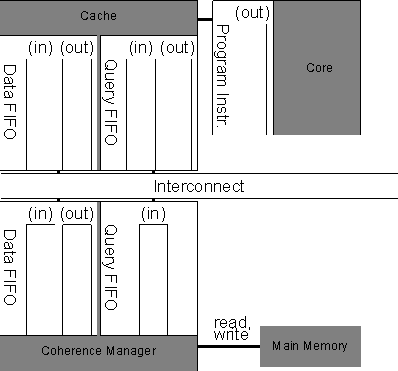
\includegraphics[width=20em]{\chapterdirectory/../cache_coherence/figure/cmp_detailed.pdf}
\caption{Vue comprenant les FIFOs}%
\label{fr:fig:cache-coherence-cmps-fifos}
\end{subfigure}
\end{tabular}
\end{center}
\caption{Composants ayant un rôle dans la cohérence de cache}%
\label{fr:fig:cache-coherence-cmps}
\end{figure}


\begin{definition}[Élément mémoire]
  \label{fr:def:memoryelement}
  La mémoire d'un système est découpée en blocs adressables.
Dans la suite, un élément mémoire correspondra directement à un bloc mémoire.
L'ensemble de tous les éléments mémoire est défini par $\memoryelements{}
\subseteq \mathbb{N}$.
\end{definition}

La cohérence de cache est activée lors des accès à des données partagées et donc lors des exécutions des
instructions d'écriture (\storeinstr{}), lecture (\loadinstr{}) et éviction (\evictinstr{}).

\begin{definition}[Programme s'exécutant sur un c\oe ur]
Les opérateurs élémentaires sont $\operators{} = \{\loadinstr{},
\storeinstr{}, \evictinstr{}, \nopinstr{}\}$ et les instructions considérées
sont
$\instructions{} = \operators{} \times \memoryelements{}$.
Un programme est une séquence d'instructions
et donc $\programs{} =
\sequenceof{\instructions{}}$.
\end{definition}
La notion de séquence sera largement réutilisée dans la suite.
\begin{definition}[Séquence]
\sequenceof{$A$} indique une séquence finie (potentiellement vide)
composée d'éléments de type $A$. Les séquences sont donc définies par:
\[
   \sequenceof{A} =
      \begin{cases}
         \lbrack ~~ \rbrack\\
         A :: \sequenceof{A}
      \end{cases}
\]
L'ajout d'un élément $e$ en tête de la séquence $S$ est noté
\pushfun{$e$}{$S$} et correspond à $e :: S$. L'extraction de la tête de la
séquence $S$ est notée \popfun{$S$}, ce qui retourne $head(S)$ avant d'appliquer
$S \gets tail(S)$. Enfin, \isemptyfun{$S$} indique si $S$ est une séquence
vide et est l'équivalent de vérifier si $S = \lbrack ~~ \rbrack$.
\end{definition}


Les caches sont chargés d'obtenir des copies des éléments mémoire afin de
répondre aux requêtes d'accès mémoire de leur cœur.


\begin{definition}[Ensemble des caches]
\label{fr:def:cache}
L'ensemble des caches du système est défini  par \caches{}.
On note $\cachesandcmgr{} = \caches{} \cup \{\cmgr{}\}$ l'ensemble des caches et le gestionnaire
de cohérence (\cmgr{}).
\end{definition}
Pour gérer les requêtes du c\oe ur,
le cache doit de stocker les
permissions sur chaque élément mémoire
et les opérations en cours.
Pour obtenir de nouvelles permissions, un cache envoie des demandes sur
l'interconnect afin de se coordonner avec les autres caches et le gestionnaire de cohérence.
Chaque demande ne concerne qu'un seul élément mémoire.
On considèrera les demandes de copie en lecture seule
de l'élément mémoire (\getsquery, faisant généralement suite à une instruction
de \loadinstr{}); de copie en écriture et lecture (\getmquery,
faisant généralement suite à une instruction de \storeinstr{}); et le signalement
d'une éviction pour un élément mémoire ayant potentiellement été modifié
(\putmquery, faisant généralement suite à un \evictinstr{}).

\begin{definition}[Demande]
Il existe trois catégories de demande $\queries{} = \{\getsquery,
\getmquery, \putmquery\}$.
Un message envoyé sur l'interconnect pour émettre une demande est défini par
$\querymessages{}: \queries{} \times \memoryelements{} \times \caches$, qui
indique le type de la demande, l'élément mémoire visé et l'émetteur du message.
\end{definition}

Chaque demande fera l'objet d'une réponse.
Une réponse peut simplement contenir une copie de l'élément mémoire (\simpledata);
une réponse peut indiquant qu'aucun autre cache ne possède actuellement de copie de cet élément
mémoire (\exclusivedata); et une réponse peut informer qu'aucune copie ne sera
envoyée (\nodata).


\begin{definition}[Réponse]
Il existe trois catégories de réponse $\replies{} =
\{\simpledata,
\allowbreak{}
\exclusivedata,\allowbreak{} \nodata\}$.
Un message envoyé sur l'interconnect pour émettre une réponse est défini par
$\replymessages{}:
\replies{} \times \memoryelements{} \times \cachesandcmgr{}$, qui indique la
catégorie, l'élément mémoire en question, et le cache visé.
\end{definition}

Il est possible que des caches reçoivent des demandes auxquelles ils doivent répondre alors qu'ils
n'ont pas encore reçu les informations nécessaires.
Ils auront donc en charge de gérer toute cette complexité et répondre à l'ensemble des requêtes et demandes qui leur sont envoyées.
Chaque cache a quatre  FIFO, chacune gérant soit la réception ou l'émission
des demandes et des réponses, comme le montre la
Figure~\ref{fr:fig:cache-coherence-cmps-fifos}.

Le gestionnaire de cohérence est un élément central, non nécessairement implanté par un composant unique dans l'architecture,
permettant la coordination entre les caches.
Tout comme les caches, il utilise des files FIFOs pour
gérer les messages entrant et sortant.
L'interconnect connecte notamment les caches et le gestionnaire de
cohérence. Il broadcast les demandes des caches à tous les composants connectés,
y compris le cache émetteur. Les réponses, quant à elles, ciblent
un seul composant et ne sont donc reçues que par celui-ci.

\subsection{Cohérence de cache}
\label{fr:sec:cache_coherence_msi}
Cette partie, inspirée des principes de \cite{Sorin:2011:PMC:2028905},
introduit la cohérence de cache.
Un système avec cohérence de cache est un système dans lequel des applications
utilisant des caches séparés ne perçoivent pas cette séparation lorsqu'elles
lisent et écrivent sur les éléments mémoire.
\begin{property}
  \label{fr:prop:system_wide_value}
Un protole doit vérifier les propriétés suivantes:
\begin{enumerate}
   \setlength{\itemsep}{0pt}%
   \setlength{\parskip}{0pt}%
  \item Les caches ont la valeur système :
    À tout moment, pour chaque élément mémoire, toutes les copies du même élément
mémoire présentes dans un cache ont la même valeur. Cette valeur correspond à
la dernière qui a été écrite pour cet élément mémoire, quel que soit le cache
qui a fait l'écriture.
  \item
    Un seul écrivain ou seulement des lecteurs :
    À tout moment, pour chaque élément mémoire, il y a soit un seul cache autorisé
à écrire et il est aussi le seul à pouvoir lire, soit aucun cache autorisé à
écrire et un nombre indéterminé de lecteurs.
\item
  Garder le fil :
Si un élément mémoire n'a pas de copie en cache, alors la valeur qui se trouve
dans la mémoire principale du système est la dernière à avoir été écrite.
\end{enumerate}
\end{property}


%\stopallthesefloats
\begin{figure}[hbtp]
   \begin{center}
     \begin{subfigure}[b]{0.5\linewidth}
       \resizebox{\linewidth}{!}{
      \begin{tikzpicture}[->,>=stealth',shorten >=1pt,auto,node distance=5cm,
                    semithick]
   \node[state] (I)              {\texttt{I}};
   \node[state] (S) [right of=I] {\texttt{S}};
   \node[state] (M) [below of=I] {\texttt{M}};

   \path[every node/.style={}]
      (I) edge [bend left] node {\textcolor{blue}{\loadinstr{}}?\textcolor{red}{\textcolor{red}{\getsquery{}}}!\textcolor{OliveGreen}{\simpledata{}}?} (S)
      (I) edge [bend right, sloped, anchor=center] node[yshift=-1em] {\textcolor{blue}{\storeinstr{}}?\textcolor{red}{\textcolor{red}{\getmquery{}}}!\textcolor{OliveGreen}{\simpledata{}}?} (M)

      (S) edge node {\textcolor{blue}{\evictinstr{}}?} (I)
      (S) edge [bend right=90, above] node {\textcolor{red}{\textcolor{red}{\getmquery{}}}?} (I)
      (S) edge [bend left, sloped, anchor=center] node[yshift=1.5em] {\textcolor{blue}{\storeinstr{}}?\textcolor{red}{\textcolor{red}{\getmquery{}}}!\textcolor{OliveGreen}{\simpledata{}}?} (M)
      (S) edge [out=430,in=400,looseness=8] node {\textcolor{blue}{\loadinstr{}}?} (S)

      (M) edge [bend left=90, above, sloped] node {\textcolor{red}{\textcolor{red}{\getmquery{}}}?\textcolor{OliveGreen}{\simpledata{}}!} (I)
      (M) edge [bend right=90, above, sloped, anchor=center] node[yshift=-1em] {\textcolor{red}{\textcolor{red}{\getsquery{}}}?\textcolor{OliveGreen}{\simpledata{}}!\textcolor{OliveGreen}{\simpledata{}}!} (S)
      (M) edge [sloped, anchor=center] node[yshift=-1em]
         {\textcolor{blue}{\evictinstr{}}?\textcolor{red}{\putmquery{}}!\textcolor{OliveGreen}{\simpledata{}}!} (I)
      (M) edge [out=230,in=200,looseness=8] node {\textcolor{blue}{\loadinstr{}}?} (M)
      (M) edge [out=280,in=250,looseness=8] node {\textcolor{blue}{\storeinstr{}}?} (M)
   ;
\end{tikzpicture}
}
      \caption{Cache}
      \label{fr:fig:general_msi_cc}
   \end{subfigure}
   \begin{subfigure}[b]{0.3\linewidth}
      \resizebox{\linewidth}{!}{
      \begin{tikzpicture}[->,>=stealth',shorten >=1pt,auto,node distance=5cm,
                    semithick]
   \node[state] (U)              {\texttt{I}};
   \node[state] (M) [left of=U] {\texttt{M}};

   \path[every node/.style={sloped, anchor=center, yshift=1em}]
      (U) edge [bend left] node {\textcolor{red}{\textcolor{red}{\getmquery{}}}?\textcolor{OliveGreen}{\simpledata{}}!} (M)
      (U) edge [loop below] node [below,yshift=-1em] {\textcolor{red}{\textcolor{red}{\getsquery{}}}?\textcolor{OliveGreen}{\simpledata{}}!} (U)

      (M) edge [bend left] node {\textcolor{red}{\putmquery{}}?\textcolor{OliveGreen}{\simpledata{}}?} (U)
      (M) edge [bend left=90] node {\textcolor{red}{\textcolor{red}{\getsquery{}}}?\textcolor{OliveGreen}{\simpledata{}}?} (U)
   ;
\end{tikzpicture}
}
      \caption{Gestionnaire de cohérence}
      \label{fr:fig:general_msi_cmgr}
   \end{subfigure}
   \begin{subfigure}[b]{0.1\linewidth}
 \resizebox{\linewidth}{!}{
     \begin{tikzpicture}[->,>=stealth',shorten >=1pt,auto,node distance=5cm,
                    semithick]
   \node[state] (U)              {};

   \path[every node/.style={sloped, anchor=center, yshift=1em}]
      (U) edge [loop left] node [below,yshift=0.5em] {\textcolor{blue}{\loadinstr{}}!} (U)
      (U) edge [loop right] node [below,yshift=-1em] {\textcolor{blue}{\storeinstr{}}!} (U)
      (U) edge [loop below] node [below,yshift=-1em] {\textcolor{blue}{\evictinstr{}}!} (U)
   ;
\end{tikzpicture}
}
      \caption{Cœur}
      \label{fr:fig:general_msi_cpu}
   \end{subfigure}
   \end{center}
   \caption{Vue d'ensemble du protocole MSI}
   \label{fr:fig:general_msi}
\end{figure}


Le protocole MSI est le protocole élémentaire de cohérence de cache
et les autres protocoles connus en sont en général des extensions.
Le protocole MSI contient trois états stables, qui lui donnent son nom:
\begin{itemize}
  \setlength{\itemsep}{0pt}%
   \setlength{\parskip}{0pt}%
\item \textbf{Modified:}
\textit{Modified}
indique qu'au moins une écriture a été réalisée sur l'élément mémoire. Tant qu'il possède une copie dans cet état, le
cache peut librement lire et écrire. Cela correspond à être l'unique écrivain
dans la Propriété~\ref{fr:prop:system_wide_value}.

\item \textbf{Shared:}
  \textit{Shared}
  correspond à un accès en lecture.

\item \textbf{Invalid:}
\textit{Invalid} indique que le cache ne possède pas de copie
de l'élément mémoire. Il ne peut donc ni le lire ni le modifier en écriture.
\end{itemize}

La Figure~\ref{fr:fig:general_msi} montre les automates correspondant
au cache, au gestionnaire et au c\oe ur. Cette vision est simplifiée
notamment car les FIFO ont été abstraites et les échanges sont synchrones.
Dans les faits, il faut distinguer les états \textit{stables}
ceux représentés ici des états
\textit{transients}, qui
représentent des étapes intermédiaires dans la résolution des demandes et des réponses.

\begin{example}%
\label{fr:ex:general_msi_single_store}
Considérons un système avec deux caches,
$C_A$ and $C_B$, et un seul élément mémoire $E$ tel que, initialement,
$C_A$ n'a pas de copie de $E$ (état \texttt{I}) et $C_B$ a une copie de $E$
dans l'état \texttt{S}. Le gestionnaire de cohérence considère donc $E$
dans l'état \texttt{I}.
Supposons que $C_A$ reçoive une requête de \storeinstr{} de son c\oe ur. Dans cette situation,
$C_A$ envoie une demande \getmquery{}, laquelle est broadcastée aux autres composants.
Voyant le \getmquery{}, $C_B$ doit alors abandonner sa copie de $E$ afin
de maintenir la Propriété~\ref{fr:prop:system_wide_value}.
De son côté, le gestionnaire de cohérence
réagit au \getmquery{} en envoyant une réponse \simpledata{} à $C_A$ et en
considérant désormais $E$ dans l'état \texttt{M}. Cette réponse
\simpledata{} permet à $C_A$ d'obtenir sa copie de $E$ avec un état \texttt{M}
et donc d'exécuter l'instruction du c\oe ur.
\end{example}




